\subsection{用户端功能实现}

用户端主要面向外卖平台中的普通消费者，提供注册登录、创建订单、订单历史查询、订单搜索、订单备注、订单通信和投诉申请等功能。用户端的设计目标是在保证用户能够顺利完成下单和通信的基础上，隐藏用户真实身份，避免将真实用户名、联系方式或 PID 直接暴露给骑手端。

用户首次使用系统时，需要在注册页面输入用户名、口令和验证码。服务器完成验证码校验、用户名唯一性检查和口令哈希存储后，为该用户生成 PID 匿名身份标识。PID 作为系统内部身份标识参与后续订单绑定和消息记录，但普通页面不长期展示 PID，骑手端也无法通过正常业务接口获取用户 PID。

\begin{figure}[H]
    \centering
    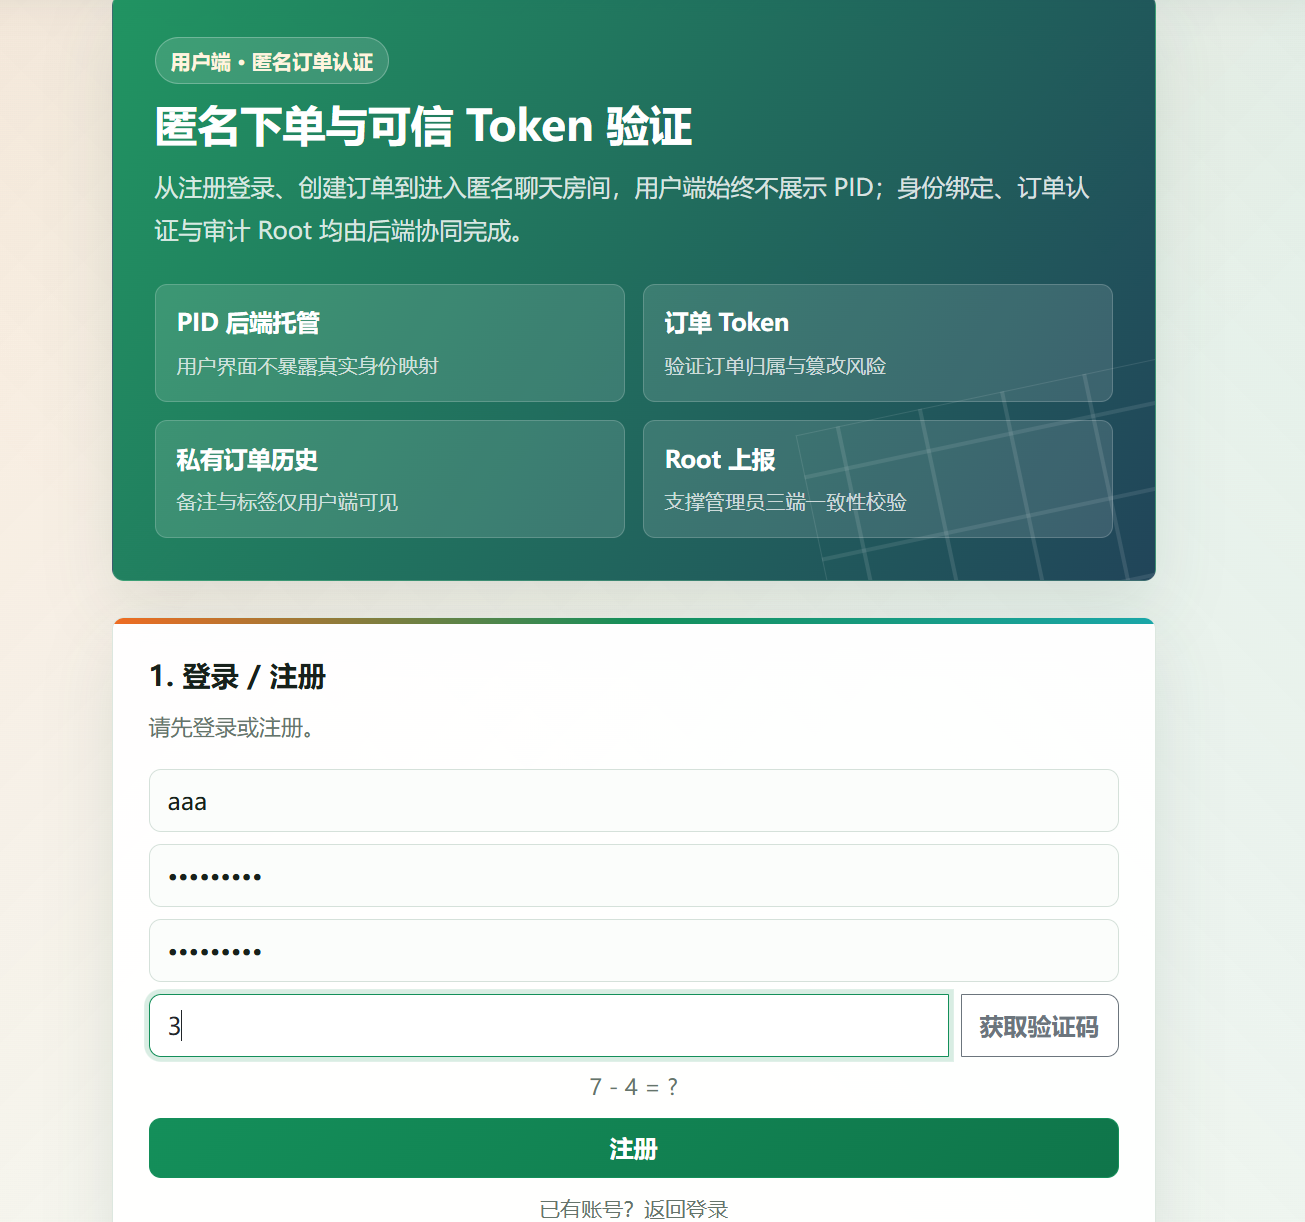
\includegraphics[width=0.85\textwidth]{content/chapter4/user_register.png}
    \caption{用户注册界面}
    \label{fig:user-register}
\end{figure}

用户登录成功后进入用户主页。用户主页提供创建订单、查看历史订单、搜索订单和进入通信页面等功能。用户创建订单时，服务器随机生成订单号，并基于订单号、用户 PID、时间戳和随机数生成订单 Token。订单创建成功后，用户端获得订单号和 Token，并可通过该凭证进入订单通信通道。

\begin{figure}[H]
    \centering
    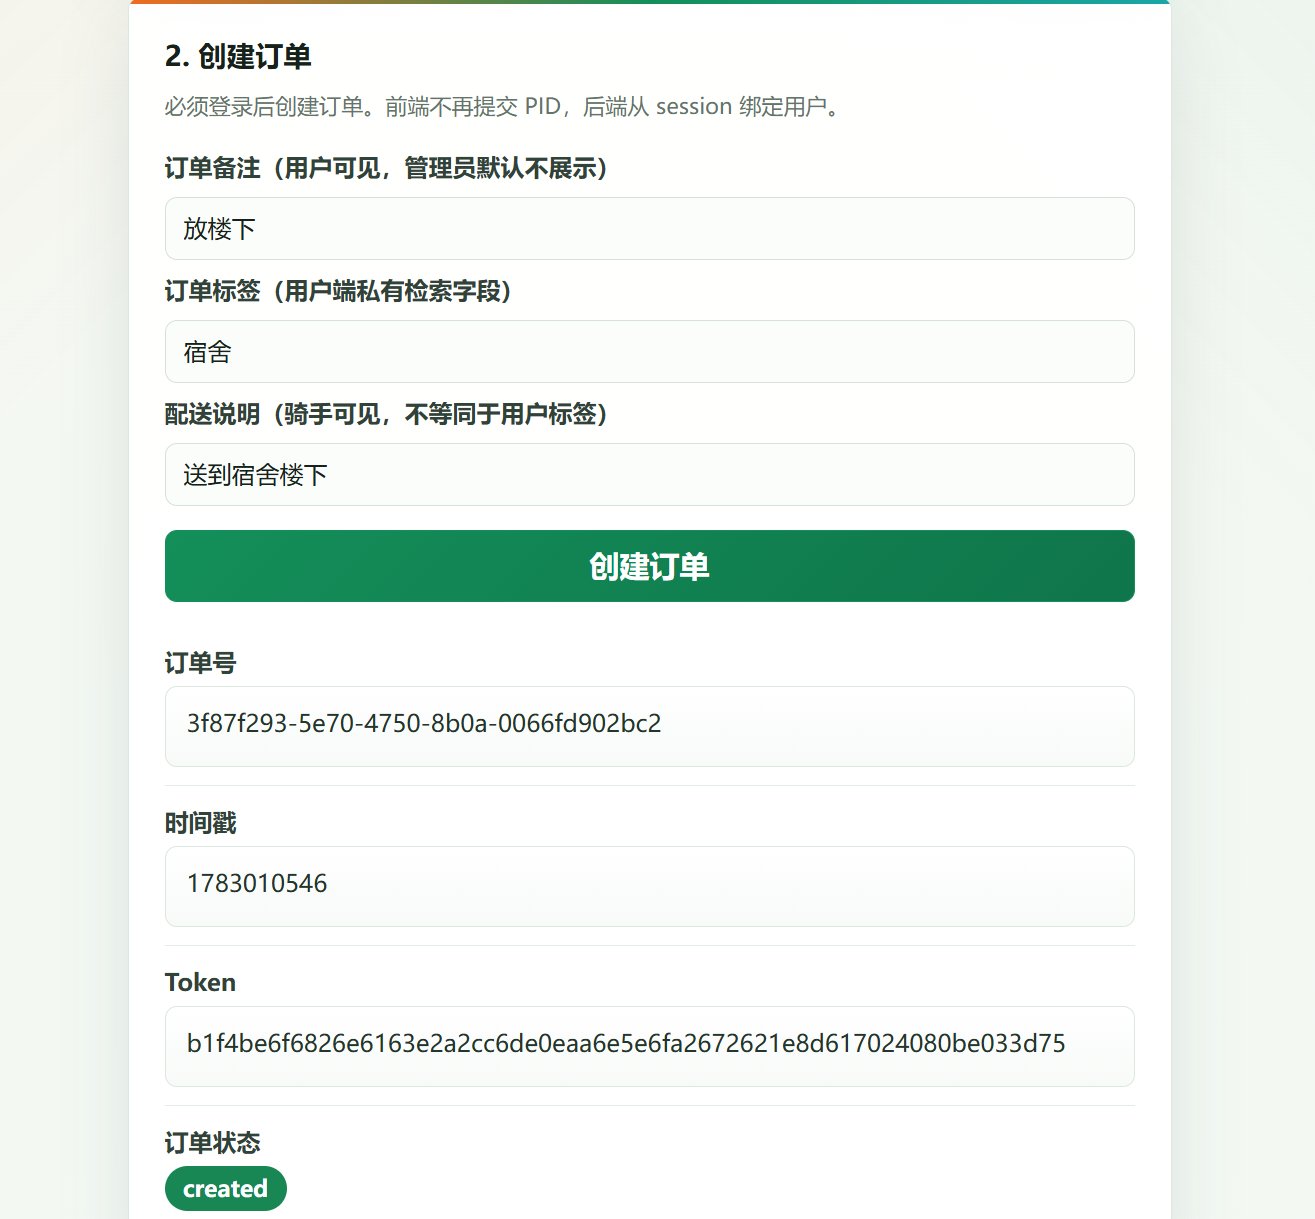
\includegraphics[width=0.85\textwidth]{content/chapter4/user_create_order.png}
    \caption{用户端订单创建界面}
    \label{fig:user-create-order}
\end{figure}

用户进入订单通信页面时，前端携带 \texttt{order\_id} 和 \texttt{token} 向服务器发起 \texttt{join\_order} 事件。服务器验证 Token 后，将该连接加入对应订单房间。通信过程中，用户输入的消息会先发送到后端，由后端完成消息编号生成、时间戳生成、SM4 加密、SM3 哈希和 Merkle Root 更新，再广播给同一订单房间中的骑手端。

\begin{figure}[H]
    \centering
    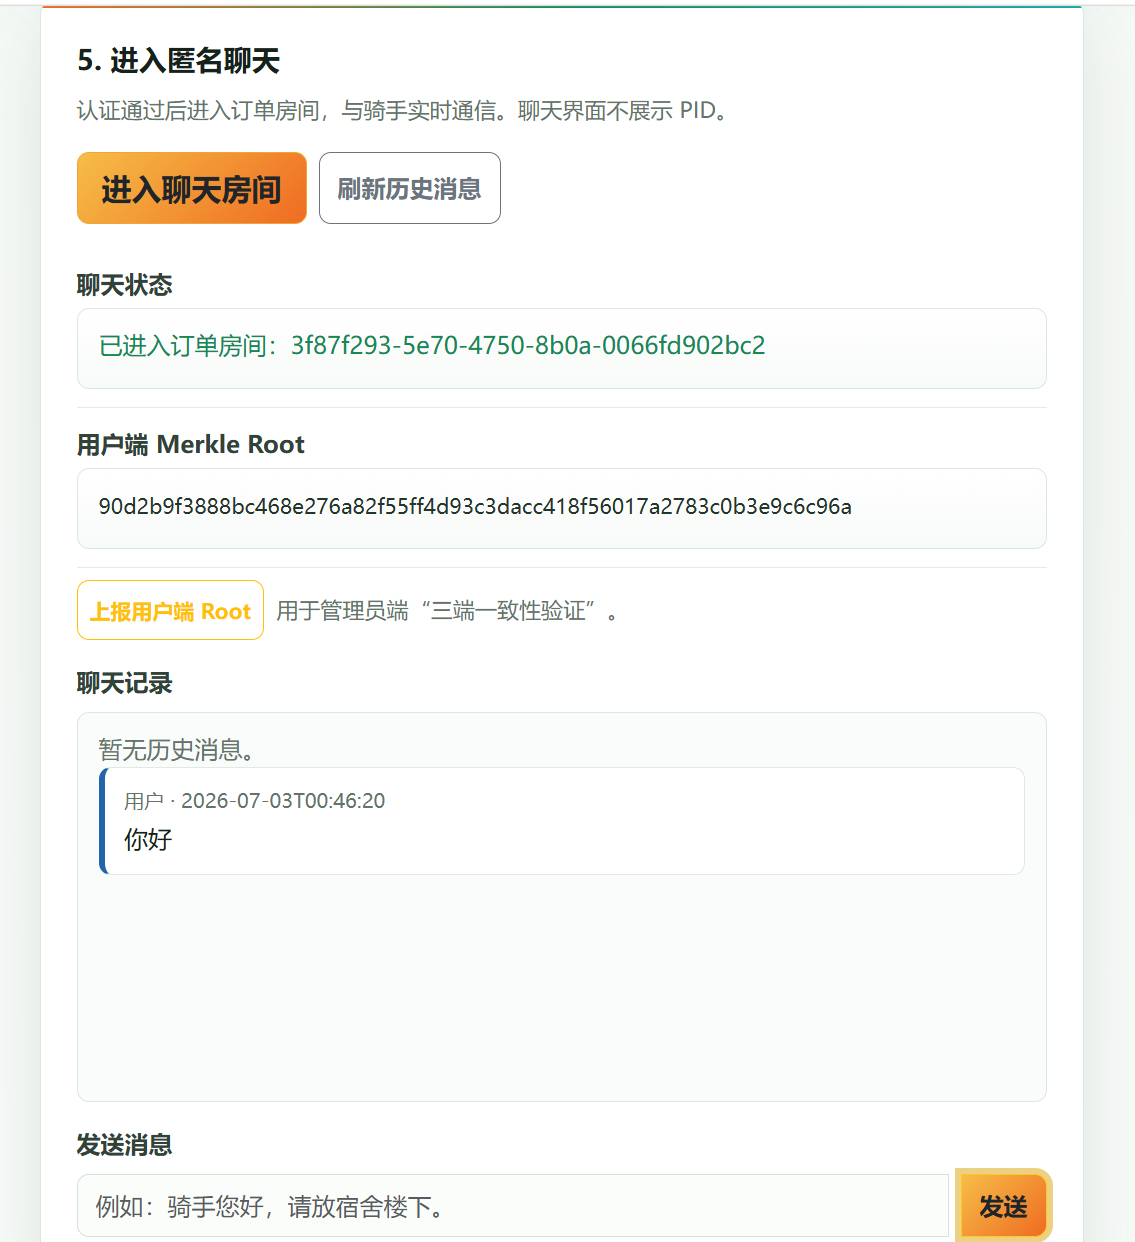
\includegraphics[width=0.9\textwidth]{content/chapter4/user_chat.png}
    \caption{用户端订单通信界面}
    \label{fig:user-chat}
\end{figure}

在异常场景下，用户端还可以基于订单号提交溯源申请。申请内容包括订单号、投诉原因和关键词。系统不允许用户直接按 PID 进行溯源申请，而是要求用户以订单号为入口提交投诉，保证溯源流程贴合外卖订单纠纷的真实业务逻辑。

\begin{figure}[H]
    \centering
    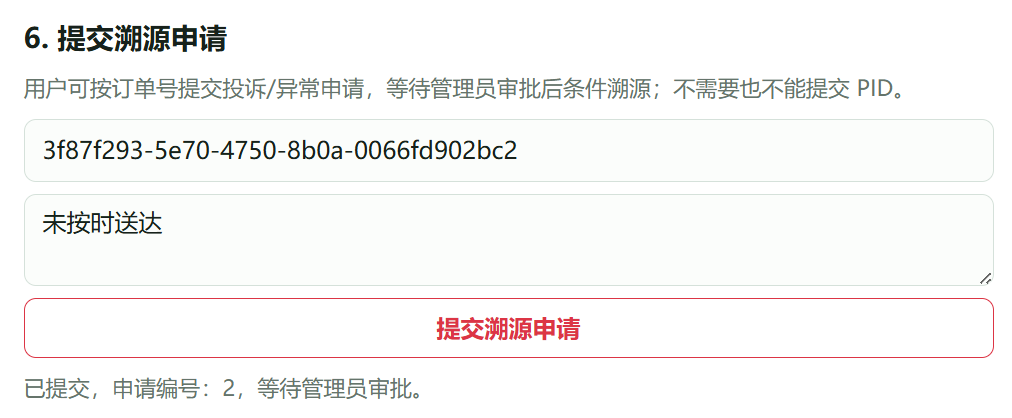
\includegraphics[width=0.85\textwidth]{content/chapter4/user_trace_request.png}
    \caption{用户端溯源申请界面}
    \label{fig:user-trace-request}
\end{figure}
